\documentclass[../Analysis-3.tex]{subfiles}

\begin{document}
\chapter*{Lecture 21} %Set chapter name
\addcontentsline{toc}{chapter}{Lecture 21} %Set chapter title
\setcounter{chapter}{21} %Set chapter counter
\setcounter{section}{0}
\setcounter{equation}{0}
\setcounter{figure}{0}

In the previous lecture, we extended our notion of Riemann integration over boxes to elementary regions. Additionally, we had discussed the change of variable formula for multivariable calculus (Theorem \ref{th:chovar}). We now try to motivate the use of the same with some rather important applications.

\section{Change of Variables (Continued)}

We start off with a particularly useful example. When dealing with functions on $\R^2$, particularly if the situation is radially symmetric, it is often useful to work in polar coordinates. Here we analyse how that change of coordinates transforms the integrals over a given region.

\begin{Eg}{Polar coordinates}{}
  \begin{wrapfigure}{r}{0.45\textwidth}
    \centering
    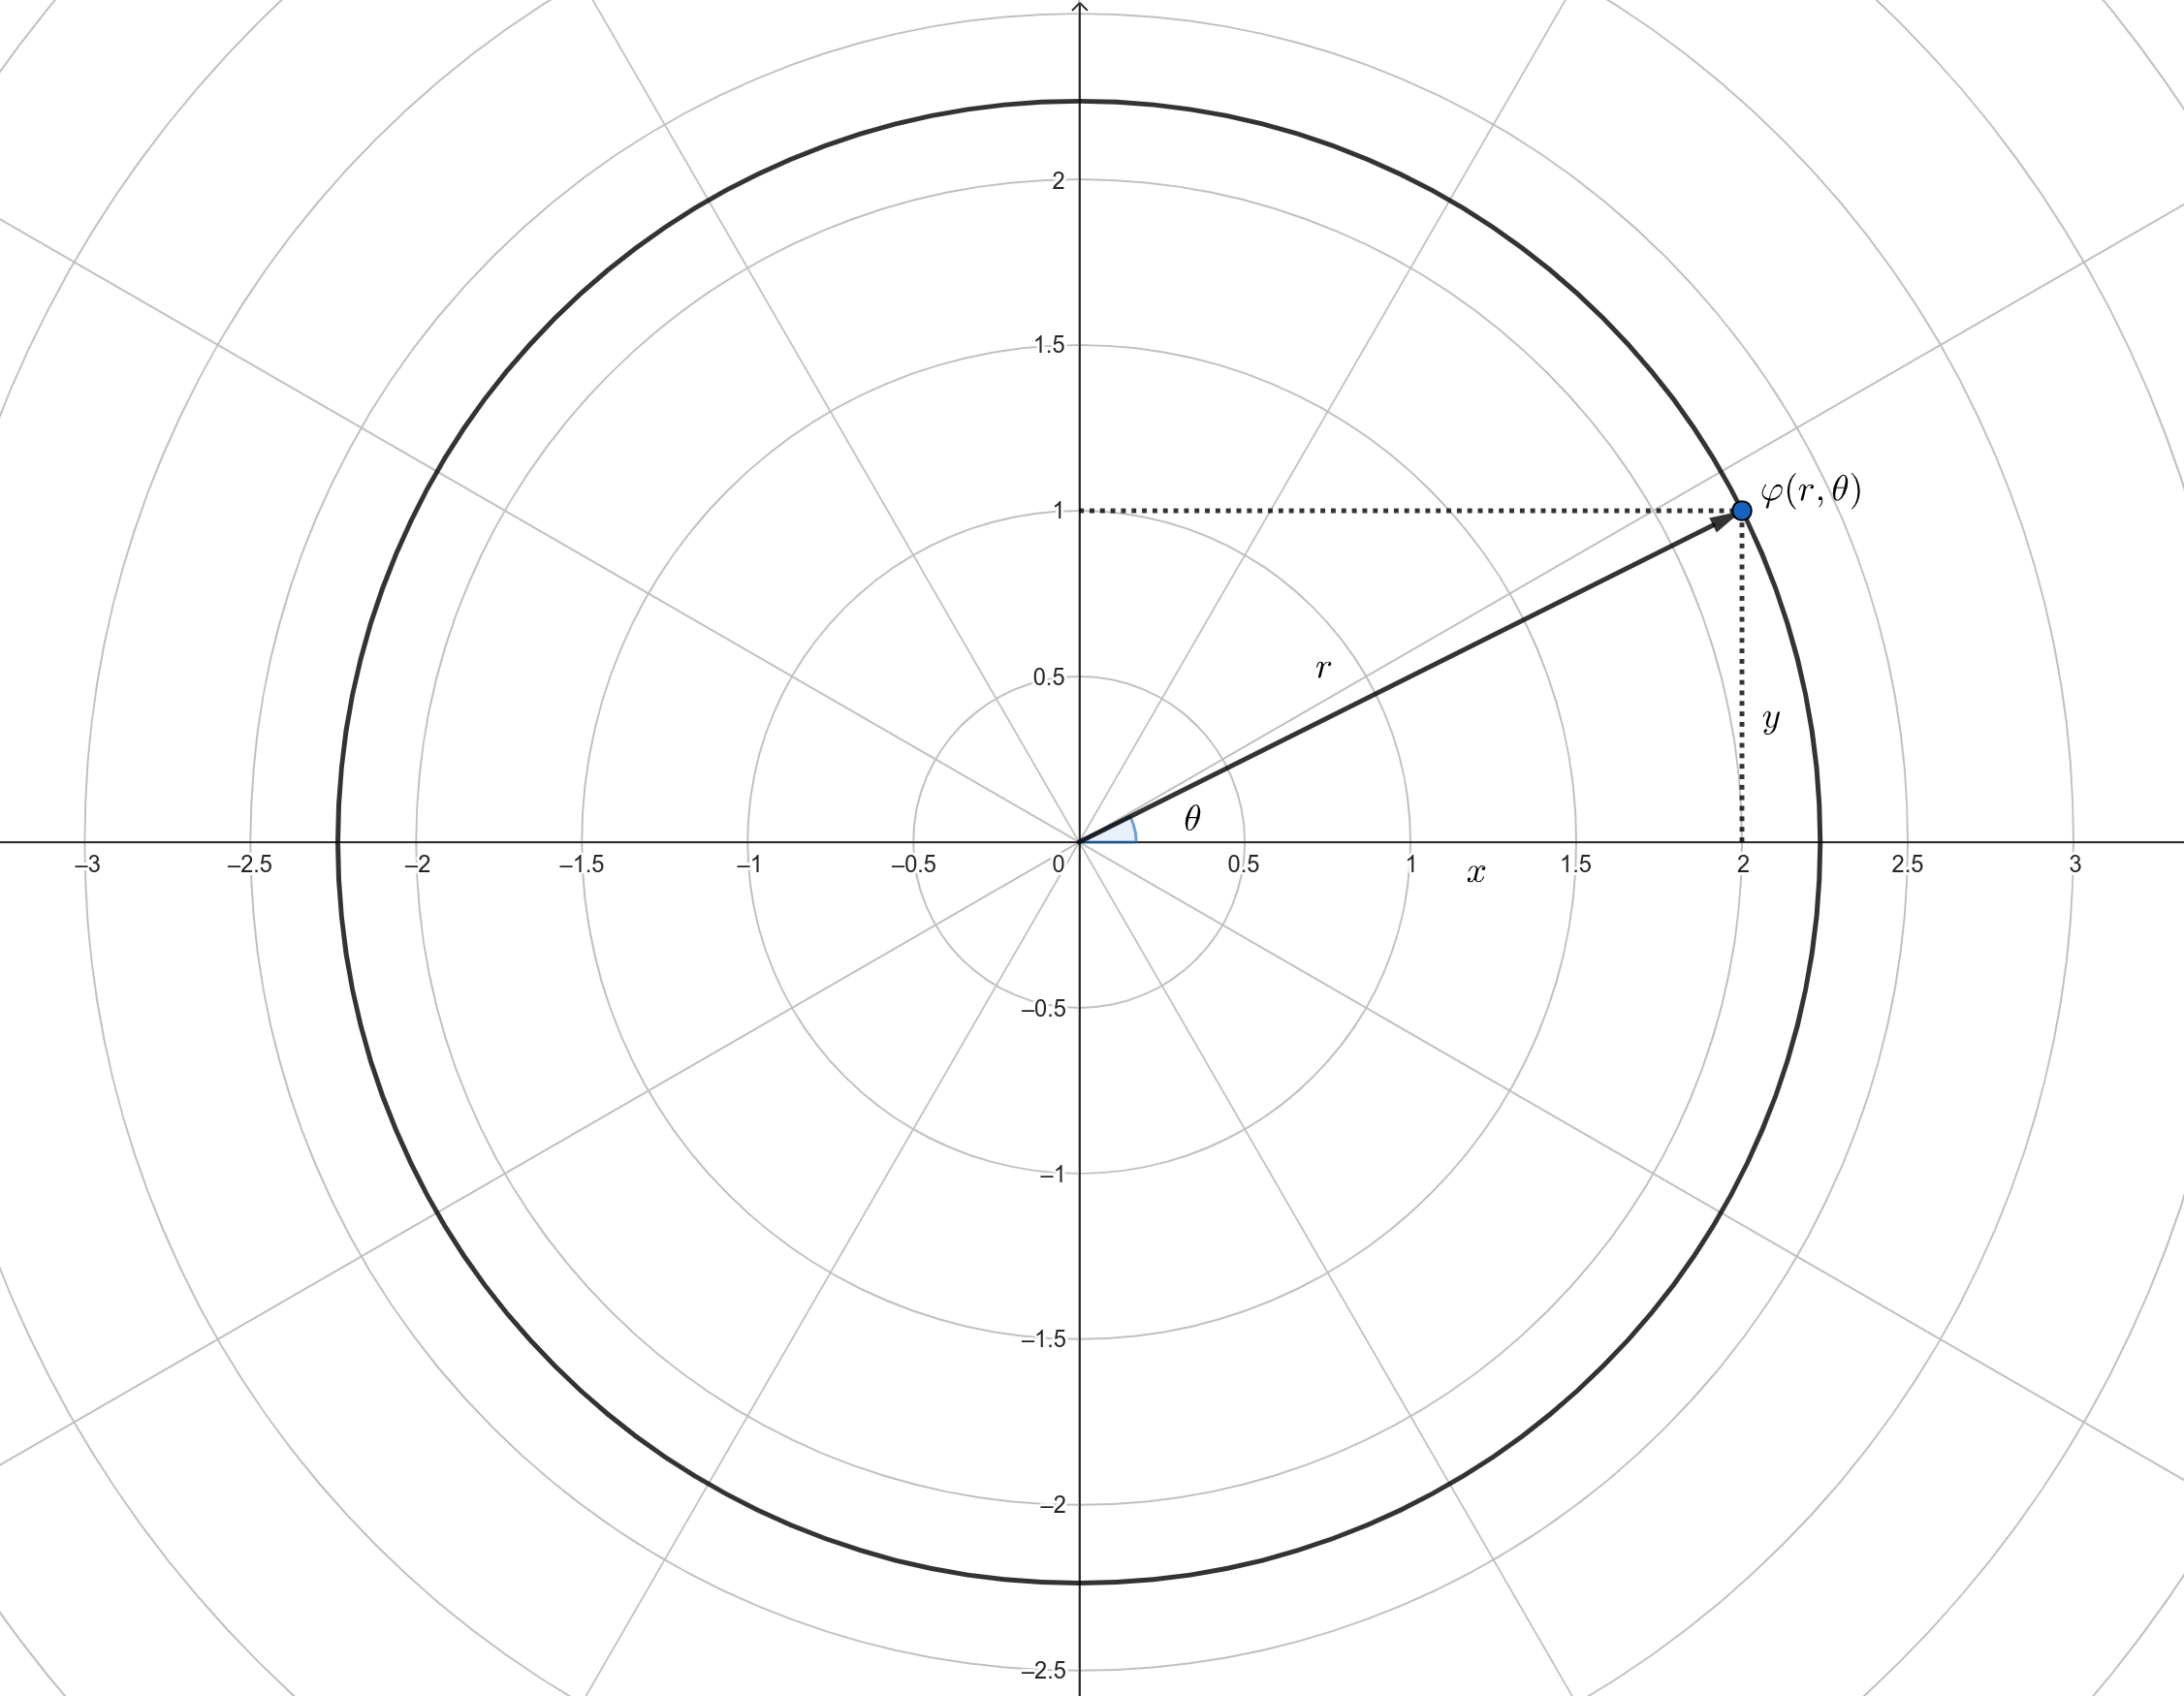
\includegraphics[width=0.5\textwidth]{../figures/lec21.1.png}
    \caption{Transforming into polar coordinates}
    \label{fig1:21}
  \end{wrapfigure}
  This example illustrates how we can compute integrals when converting to polar coordinates from Cartesian coordinates.\\
  Consider $\varphi : \R^2 \to \R^2$ given by $\varphi(r,\theta) = (r \cos\theta, r \sin\theta)$. Then, the Jacobian matrix of $\varphi$ is given by
  \[
    J_{\varphi}(r,\theta) = \begin{pmatrix}
      \cos\theta & -r\sin\theta \\
      \sin\theta & r\cos\theta
    \end{pmatrix}
  \]

  Thus, $\det(J_{\varphi}(r,\theta)) = r \neq 0 $ for all $r>0$. Taking the domain to be $\mathcal{O}_2 := (0,\infty) \times (0,2\pi)$, the function $\varphi\vert_{\mathcal{O}_2} : \mathcal{O}_2 \to \R^2$ is $C^1$ and injective, with $\det(J_{\varphi}(r,\theta)) \neq 0 $. For some fixed $0 < r_1 < r_2$ and $0 \leq \theta_1 < \theta_2 < 2\pi$, consider the set $\Omega = (r_1, r_2) \times (\theta_1, \theta_2)$. Clearly the boundary $\partial \Omega$ is of content zero (since it is union of finitely many line segments) and thus using Theorem \ref{th:chovar} we see that for $f \in \mathscr{R}(\varphi(\Omega))$,
  \begin{align*}
    \int_{\varphi(\Omega)} f
     & = \int_{\Omega} (f \circ \varphi) |\det (J_{\varphi}(r,\theta))|                                 \\
     & = \int_{\Omega} r f(r\cos\theta, r\sin\theta)                                                    \\
     & = \int_{r_1}^{r_2} \int_{\theta_1}^{\theta_2} r f(r\cos\theta, r\sin\theta)\, \dd\theta \, \dd r
  \end{align*}

  As a simple example, consider the following integral:
  \[
    \int_{x^2 + y^2 < 1} e^{-(x^2+y^2)} \dd A
  \]

  The domain of integration can be written as
  \[
    \{ (x,y) \mid x^2 + y^2 < 1 \} = \varphi( (0,1) \times [0,2\pi))
  \]

  Clearly $f(x,y) = e^{-(x^2+y^2)} \in C^1(\varphi((0,1) \times [0,2\pi)))$ which shows that:
  \begin{align*}
    \int_{x^2+y^2 < 1} e^{-(x^2+y^2)} \, \dd A
     & = \int_0^1 \left( \int_0^{2\pi} re^{-r^2} \, \dd \theta \right) \dd r \\
     & = 2\pi \int_0^1 r e^{-r^2} \, \dd r                                   \\
     & = \pi \left( 1 - \frac{1}{e}\right)
  \end{align*}
\end{Eg}

\begin{Def}{Area or volume of a region}{}
  For $\Omega \subseteq \R^n$, the volume of the region $\Omega$ is defined by the integral
  \[
    \int_{\R^n} \chi_{_\Omega}
  \]
  if it exists, where $\chi_{_\Omega}$ is the indicator function of the region $\Omega$, given by
  \[
    \chi_{_\Omega} = \begin{cases}
      1 & \mbox{ if } x \in \Omega, \\
      0 & \mbox{ otherwise}.
    \end{cases}
  \]
  
\end{Def}

\begin{Eg}{}{}
  Compute the area of $\Omega = \left\{ (x,y) \mid x^{\frac{2}{3}} + y^{\frac{2}{3}} < 1 \right\}$. Consider the function
  \begin{align*}
    \varphi : [0,1] \times [0,2\pi] & \to \R^2                                 \\
    (r,\theta)                      & \mapsto ( r\cos^3\theta, r\sin^3\theta )
  \end{align*}
  then clearly $\varphi([0,1] \times [0,2\pi]) = \Omega$. Also $\varphi$ is injective and $C^1$, but we have
  \[
    \det(J_{\varphi}(r,\theta)) = 3r \sin^2\theta \cos^2\theta
  \]
  and thus $\det(J_{\varphi}(r,\theta)) = 0$ if $r = 0$ or $\theta \in \left\{ 0, \frac{\pi}{2}, \pi, \frac{3\pi}{2}, 2\pi \right\}$, but set of all such points are of content zero, hence we can safely ignore them while doing our integration. We get
  \begin{align*}
    \mbox{ Area of } \Omega
     & = \mbox{ Area of } \varphi \left( [0,1] \times [0,2\pi] \right)              \\
     & = \int_{\varphi([0,1] \times [0,2\pi])} 1 \, \dd A                           \\
     & = \int_0^1 \int_0^{2\pi} \frac{3}{4} r \sin^2 2\theta \, \dd \theta \, \dd r = \frac{3\pi}{8}
  \end{align*}
\end{Eg}

Next up, consider a change of coordinates in $\R^3$, from Cartesian system to the spherical co-ordinate system. Just like the previous case, this comes in handy when dealing with functions and regions which are spherically symmetric. One canonical example may be its use in the theory of central forces in physics.

\begin{Eg}{Spherical coordinates}{}
  \begin{wrapfigure}{l}{0.45\textwidth}
    \centering
    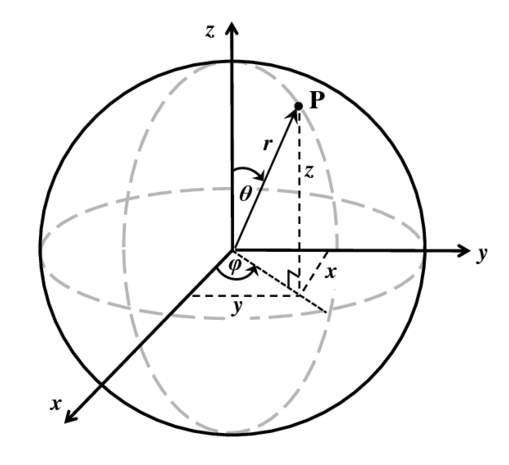
\includegraphics[width=0.45\textwidth]{../figures/lec21.2.png}
    \caption{Transforming into spherical coordinates}
    \label{fig2:21}
  \end{wrapfigure}
  The spherical co-ordinate system gives a unique representation to all points in $\R^3$ not lying on the $z$-axis. For all $(x,y,z) \in \R^3 \setminus \{ (0,0,\alpha) \mid \alpha \in \R \}$, set
  \[
    (x,y,z) = (r\sin\phi\cos\theta, r\sin\phi\sin\theta, r \cos\phi)
  \]
  where $r>0$, $0 < \theta < 2\pi$ and $0 < \phi < \pi$. Define the set \[
    \mathcal{O}_3 := \left\{ (r,\phi,\theta) \mid r >0, \, 0 < \phi < \pi \mbox{ and } 0 < \theta < 2\pi \right\}
  \]
  and the map
  \begin{align*}
    \varphi : \mathcal{O}_3 & \to \R^3, \ \varphi(r,\phi,\theta) = (x,y,z)
  \end{align*}
  Then, the Jacobian matrix of the map $\varphi$ is:
  \[
    J_{\varphi}(r,\phi,\theta) = \begin{pmatrix}
      \sin\phi\cos\theta & r\cos\phi\cos\theta & -r\sin\phi\sin\theta \\
      \sin\phi\sin\theta & r\cos\phi\sin\theta & r\sin\phi\cos\theta  \\
      \cos\phi           & -r\sin\phi          & 0
    \end{pmatrix}
  \]


  This gives $\det(J_{\varphi}(r,\phi,\theta)) = r^2 \sin \phi$, which is non-vanishing in the given domain. As $\varphi$ is injective and $C^1$, we can use Theorem \ref{th:chovar} to transform from Cartesian to spherical coordinates. We provide a simple example for some clarity.\\

  Consider the solid sphere of radius $a$, given by $\Omega = \{ (x,y,z) \mid x^2 + y^2 + z^2 \leq a^2 \}$. Then, the volume is:
  \begin{align*}
    \Vol(\Omega)
     & = \int_0^{2\pi}\int_0^{\pi} \int_0^a r^2 \sin \phi \, \dd r \, \dd \phi \, \dd \theta \\
     & = \frac{4}{3}\pi a^3
  \end{align*}
\end{Eg}

We leave it to the reader to do a similar analysis for the cylindrical co-ordinate system. This formula also finds extensive use in probability theory, where it is commonly referred to as the change of density formula (see, for instance \textit{A First Course in Probability} by Sheldon Ross, or any introductory probability book for that matter). Hopefully, we have demostrated to the reader the central role Theorem \ref{th:chovar} plays in analysis of several variables, enough to convince him to actually read the proof! We will now depart from the general study of functions and integrals in $\R^n$, and delve into the theory of curves and surfaces, dealing primarily with $\R^3$.
\end{document}
